\documentclass[11pt, a4paper]{article}

\usepackage[T1]{fontenc}
\usepackage[latin9]{inputenc}
\usepackage[english]{babel}
\usepackage{hyperref}
\usepackage{setspace}
\usepackage{graphicx}

\title{Pinned Down}
\author{Nick Pruehs}

\begin{document}

\maketitle

\onehalfspacing

\tableofcontents

\section{Introduction}

In \emph{Pinned Down}, the players command a small fleet carrying the last
survivors of the known universe: An ancient, unknown, and aggressive race has
entered their dimension, seeking to destroy all younger races that might become
a threat to them and will not cease attacking until their enemies are completely
eradicated.

The players need to work together in order to survive until they find a safe
harbor to live in peace.

\section{Goal}

The players win if they succeed in carrying out enough jumps to cover a distance
of ten or more. They lose if all of their flagships are destroyed, or if any
card explicitly says so.

\section{Affiliations}
\subsection{Purple Wing}

The main tasks of purple wing are recon and covert ops. Their ships excel at
scouting unknown space and enemy fleet movements while hiding the whole fleet
from enemy sensors.

\begin{itemize}
 \item peeking at the top cards of the attack deck
 \item peeking at the top cards of the location deck
 \item threat control
 \item cloaking
\end{itemize}

\subsection{Red Wing}

The red wing makes up the military backbone of the fleet. Their cruisers and
battleships provide the firepower required for facing any possible enemy.

\begin{itemize}
 \item fighting
\end{itemize}

\subsection{Blue Wing}

The whole fleet is supported by the men and women aboard the blue wing's ships.
It's them who ensure that the fleet doesn't fall apart and that most of them
will reach their destination in one piece.

\begin{itemize}
 \item repairing
 \item retrieving cards from the discard pile
\end{itemize}

\subsection{Ac'arr}

The Ac'arr swarm has joined the fleet in order to avert distincion. Their
diversification and ability to adapt enables them to face any imaginable threat.

\begin{itemize}
 \item no characters or equipment
 \item all ships share game texts
\end{itemize}

\section{Most Basic Rule}

A card's game text takes precedence over these rules. Always.

\section{Card Piles}

The cards of this game are kept in different piles throughout a match. Every
player has a draw deck, a hand and a discard pile.

At the beginning of the game, all cards of a player's deck go to his or her
\emph{draw deck}. Players may not have a look at their draw deck unless a card
allows them to. Whenever a player draws a card, that card is drawn from the top
of the draw deck.

The \emph{hand} of each player contains the cards he or she may play during the
main phase (or during the attack phase in case of some effects). Players may
show their hands to each other whenever they want to. There's no limit on the
number of cards in a player's hand.

Every time a player is forced to discard a card, either from play or from his or
her hand, that card goes to that player's \emph{discard pile}. All player ships
that are destroyed in battle go to their owning player's \emph{destroyed pile}.
No player may play copies of unique ships in destroyed piles. Players may have a
look at their discard and destroyed piles at any time.

The \emph{attack deck} contains all cards that represent the opposition the
players have to face. The players must not look at the cards in the attack deck
at any time unless a card allows them to.

Whenever an attack event or an attacking starship is discarded, that card is put
on the \emph{attack discard pile}. If a card needs to be drawn from the attack
deck and the attack deck is empty, the attack discard pile is shuffled and makes
up the new attack deck.

The \emph{location deck} contains all possible locations the players may jump
to. At the end of each turn, they have to decide which location to jump to in
order to get closer to their goal. Players may not have a look at the location
deck unless a card allows them to.

Every time a player starship is damaged, cards in the \emph{damage deck} tell
how the attributes of that starship are affected, and if the ship is finally
destroyed, or not. Discarded damage cards go to the \emph{damage discard pile}.
If any ship is damaged and the damage deck is empty, the damage discard pile
is shuffled turned face down, making up the new damage deck.

\section{Game Setup}

At the very beginning, the players perform the following actions to prepare the
game:

\begin{enumerate}
  \item Every player puts his or her flagship into play (for free).
  \item Every player shuffles his or her draw deck and draws four cards.
  \item The players shuffle the attack, location and damage decks.
\end{enumerate}

\section{Card Types}

Each card has a \emph{name}, a \emph{picture} and a \emph{type}. The different
card types are explained below. A card's \emph{game text} can have significant
impact on the game and always takes precedence over these rules.

Most cards have a \emph{threat} value indicated at the top-left corner. If
players play any card, they have to add that amount of threat tokens to the
threat pool. This threat is used for determining the strength of the opposition
they have to face during the attack phase.

The top-right corner of the card features the \emph{affiliation icon} of the
affiliation the card belongs to. Players can mix the cards of all affiliations
if they want to; however, most cards of an affiliation affect only that
affiliation.

The \emph{card lore}, \emph{index} and \emph{copyright note} have no effect on
the game.

\subsection{Characters}

Characters can be deployed to any starship of any player's fleet and provide
special abilities like playing cards from the draw deck or retrieving cards from
the discard pile. They can move to any other player starship on the table.

\begin{figure}
  \centering
  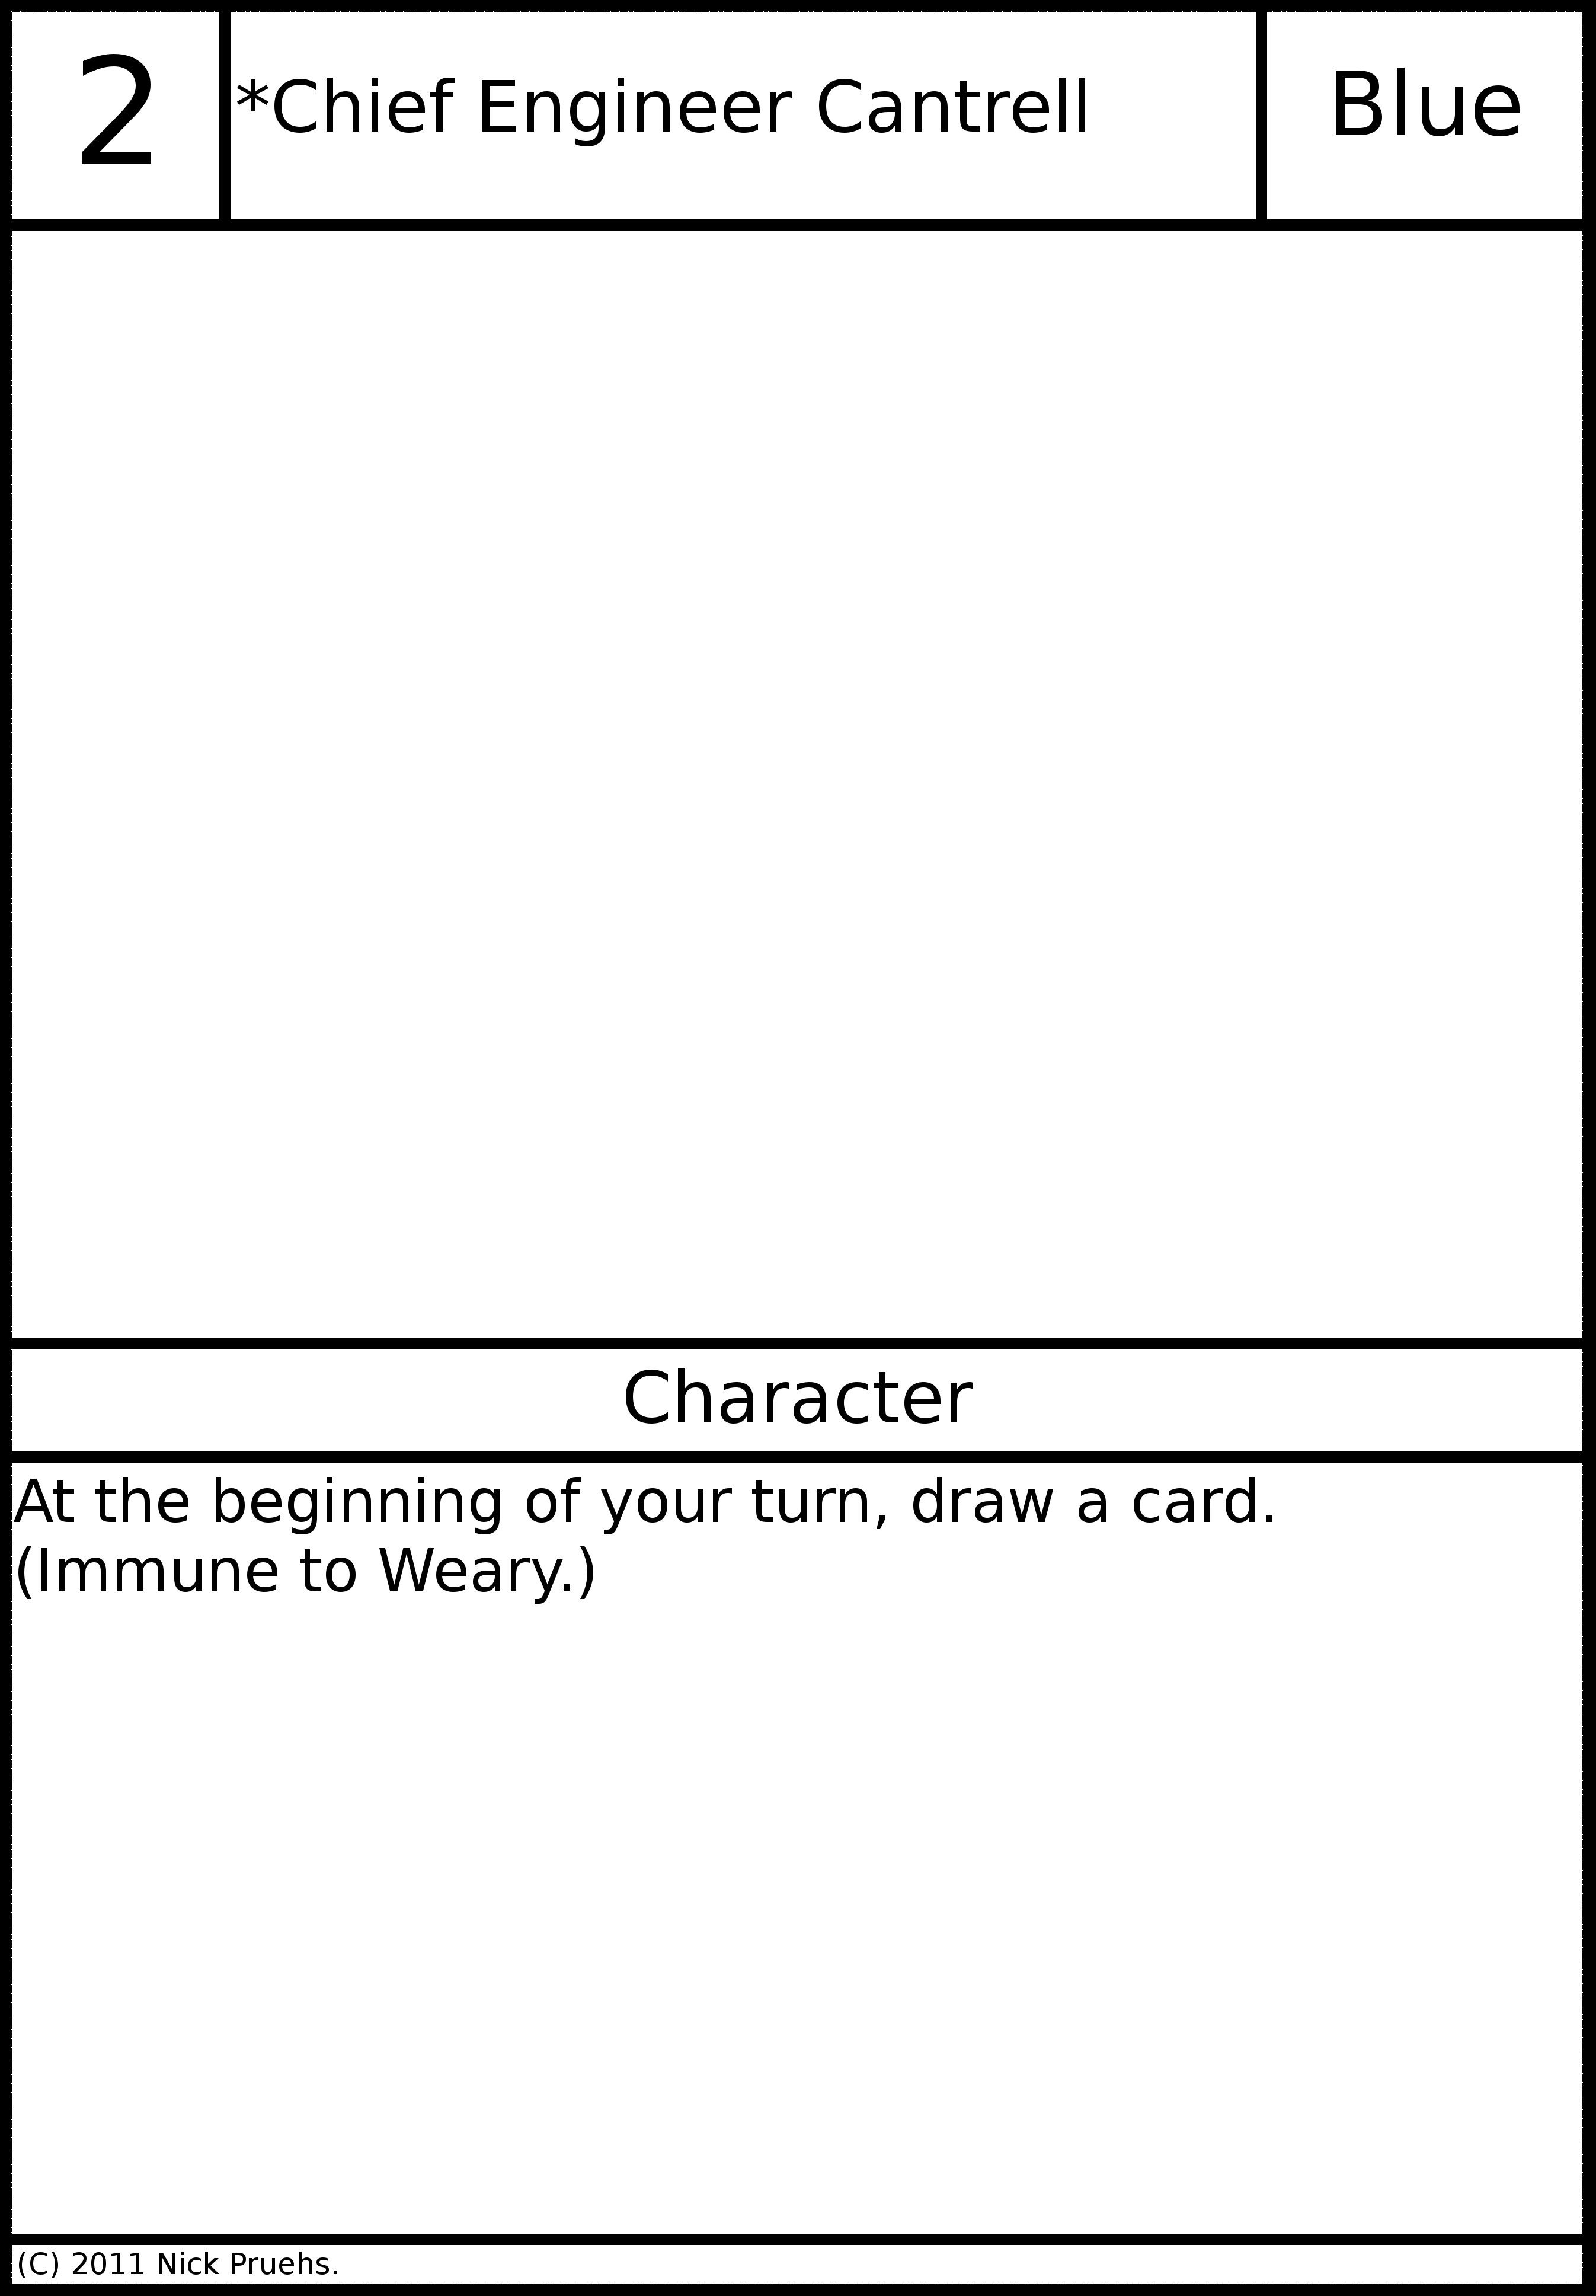
\includegraphics[width=0.5\textwidth]{examplecharacter.png}
  \caption{A character card.}
\end{figure}

Some characters are \emph{captains} of specific starships: They increase the
power of their ships by two while aboard.

\subsection{Effects}

Effects may be played at any time if they don't add threat. Effects with a
threat value greater than zero may only be played during the main phase.

\begin{figure}
  \centering
  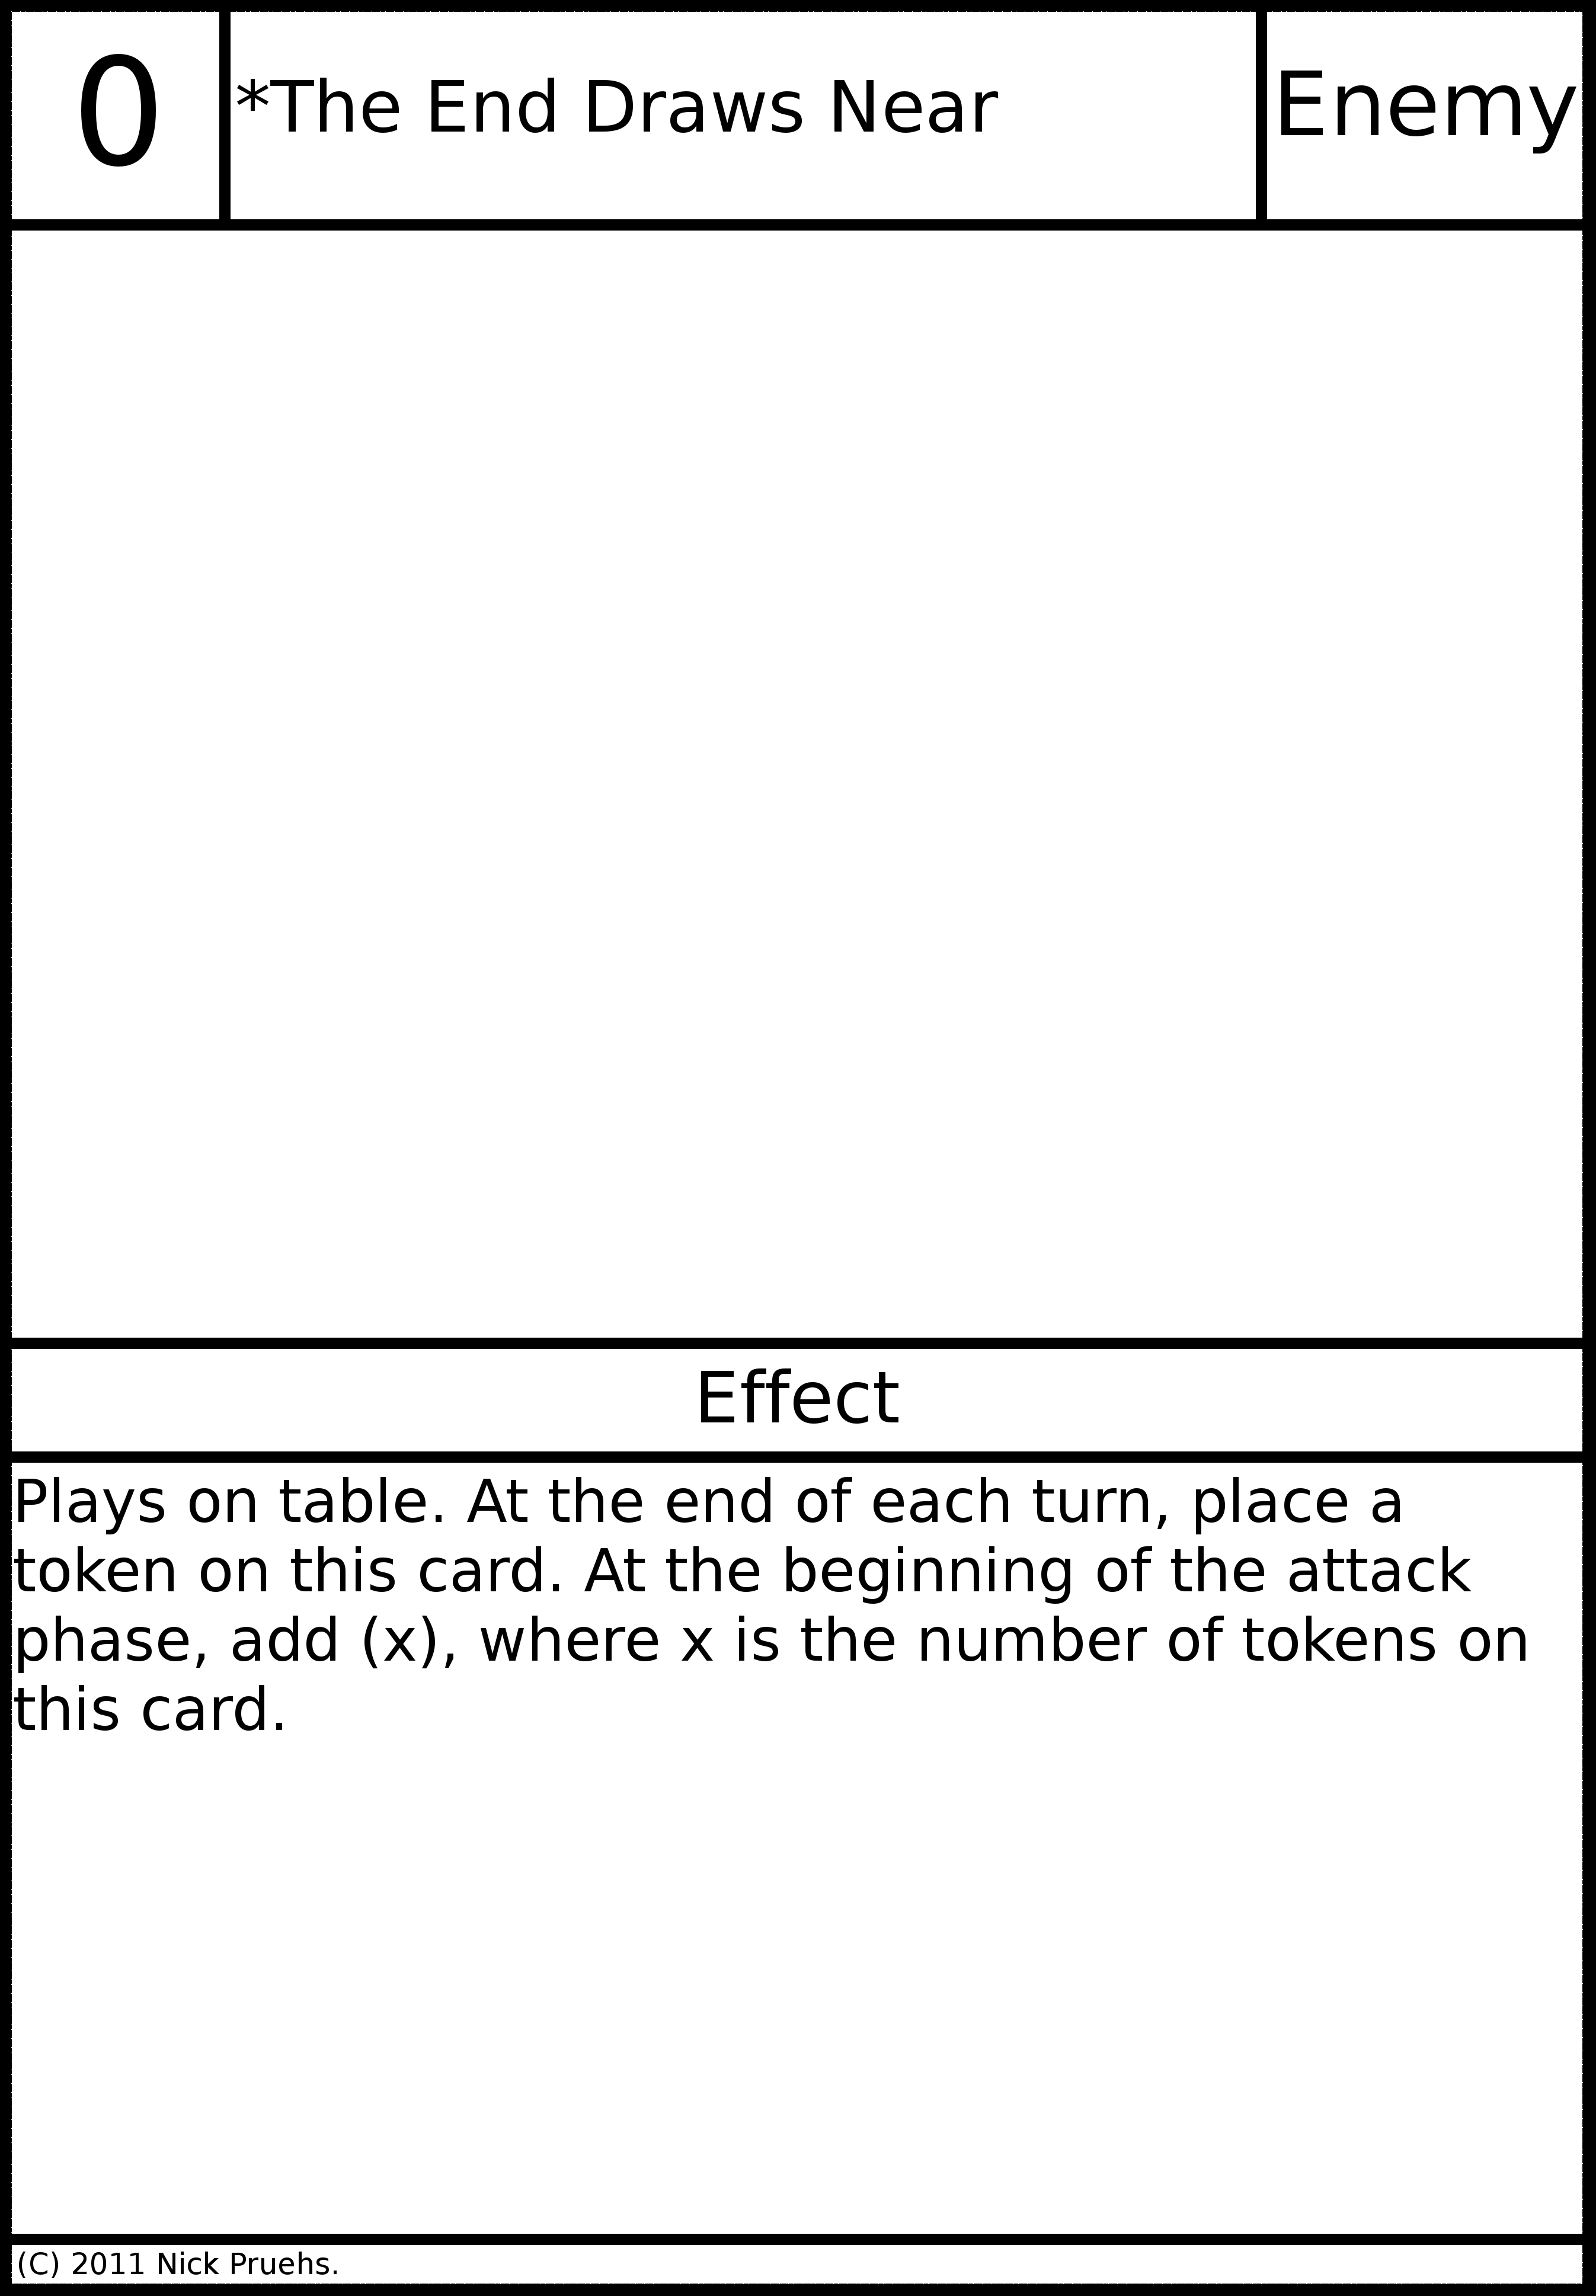
\includegraphics[width=0.5\textwidth]{exampleeffect.png}
  \caption{An effect card.}
\end{figure}

All effects take effect immediately and are discarded afterwards, unless they
state otherwise.

\subsection{Equipment}

Just like characters, equipment cards can be deployed to any starship of a
player's fleet, and they can move to any other player starship. They usually
enhance the ship they're aboard in some way.

\begin{figure}
  \centering
  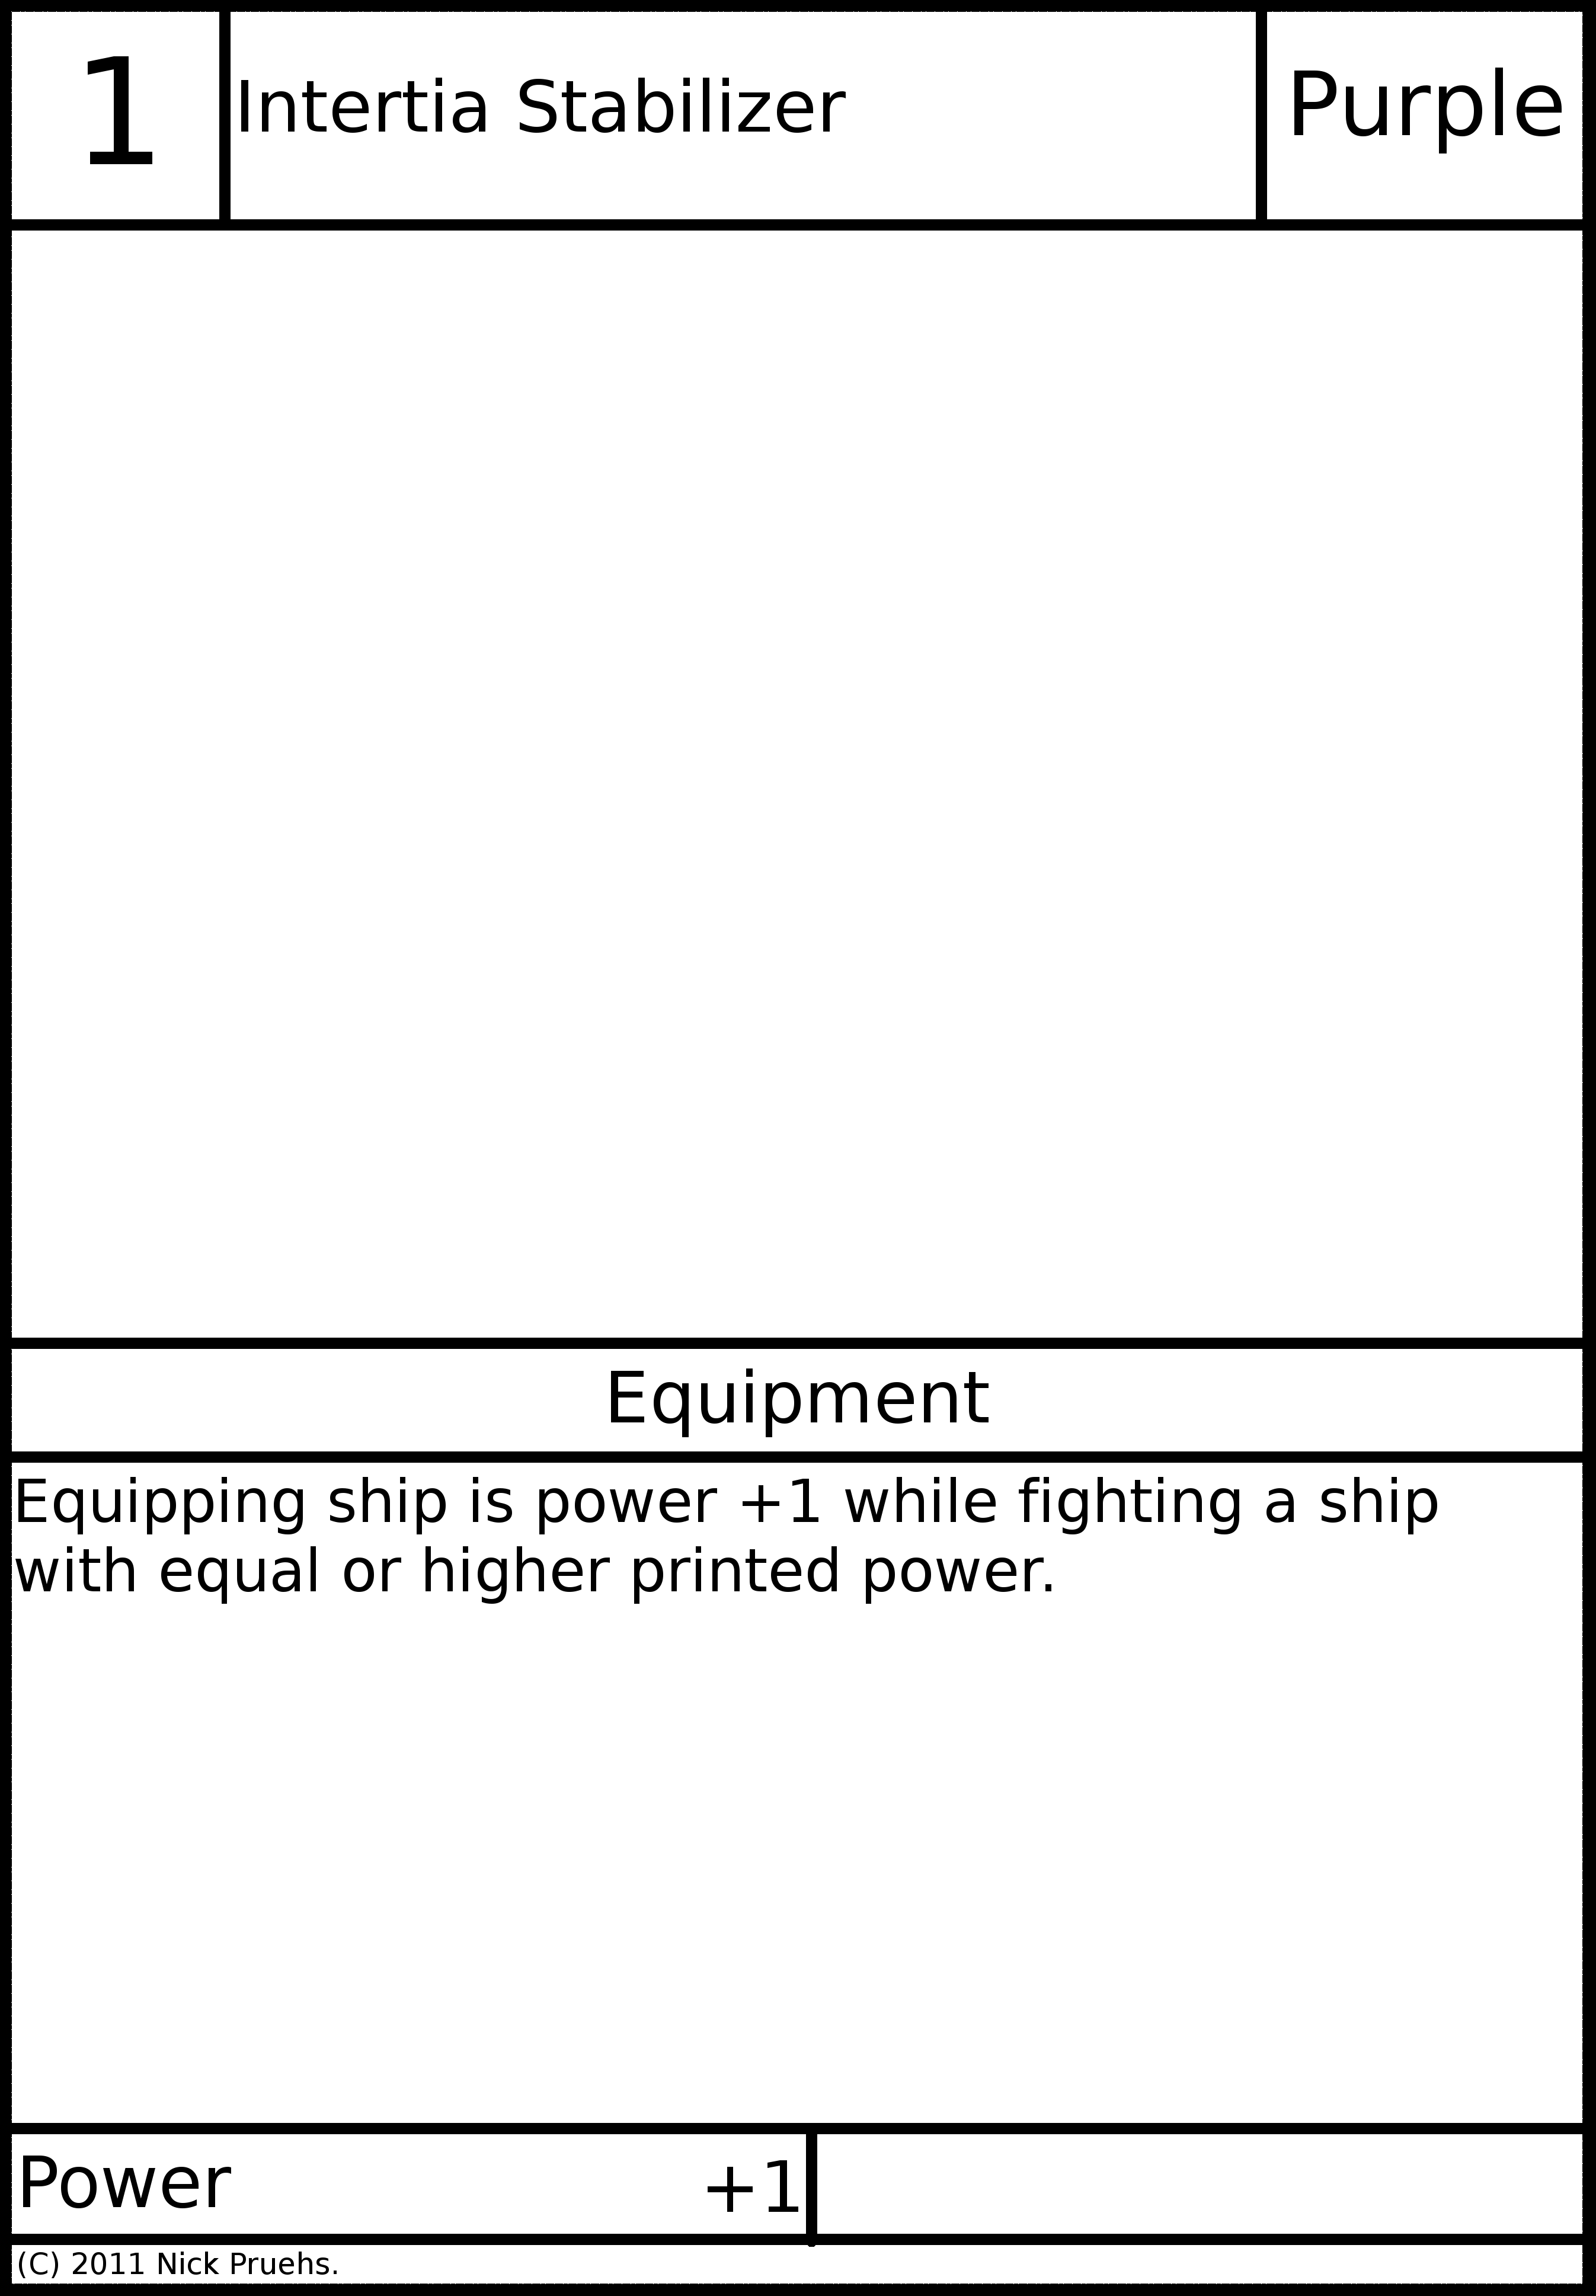
\includegraphics[width=0.5\textwidth]{exampleequipment.png}
  \caption{An equipment card.}
\end{figure}

\subsection{Starships}

Starships are required to face the enemy attacks every turn. They use their
\emph{power} value to fight against attacking ships during the attack phase.
Starships can carry the number of characters and/or equipment cards specified by
their \emph{capacity} value.

\begin{figure}
  \centering
  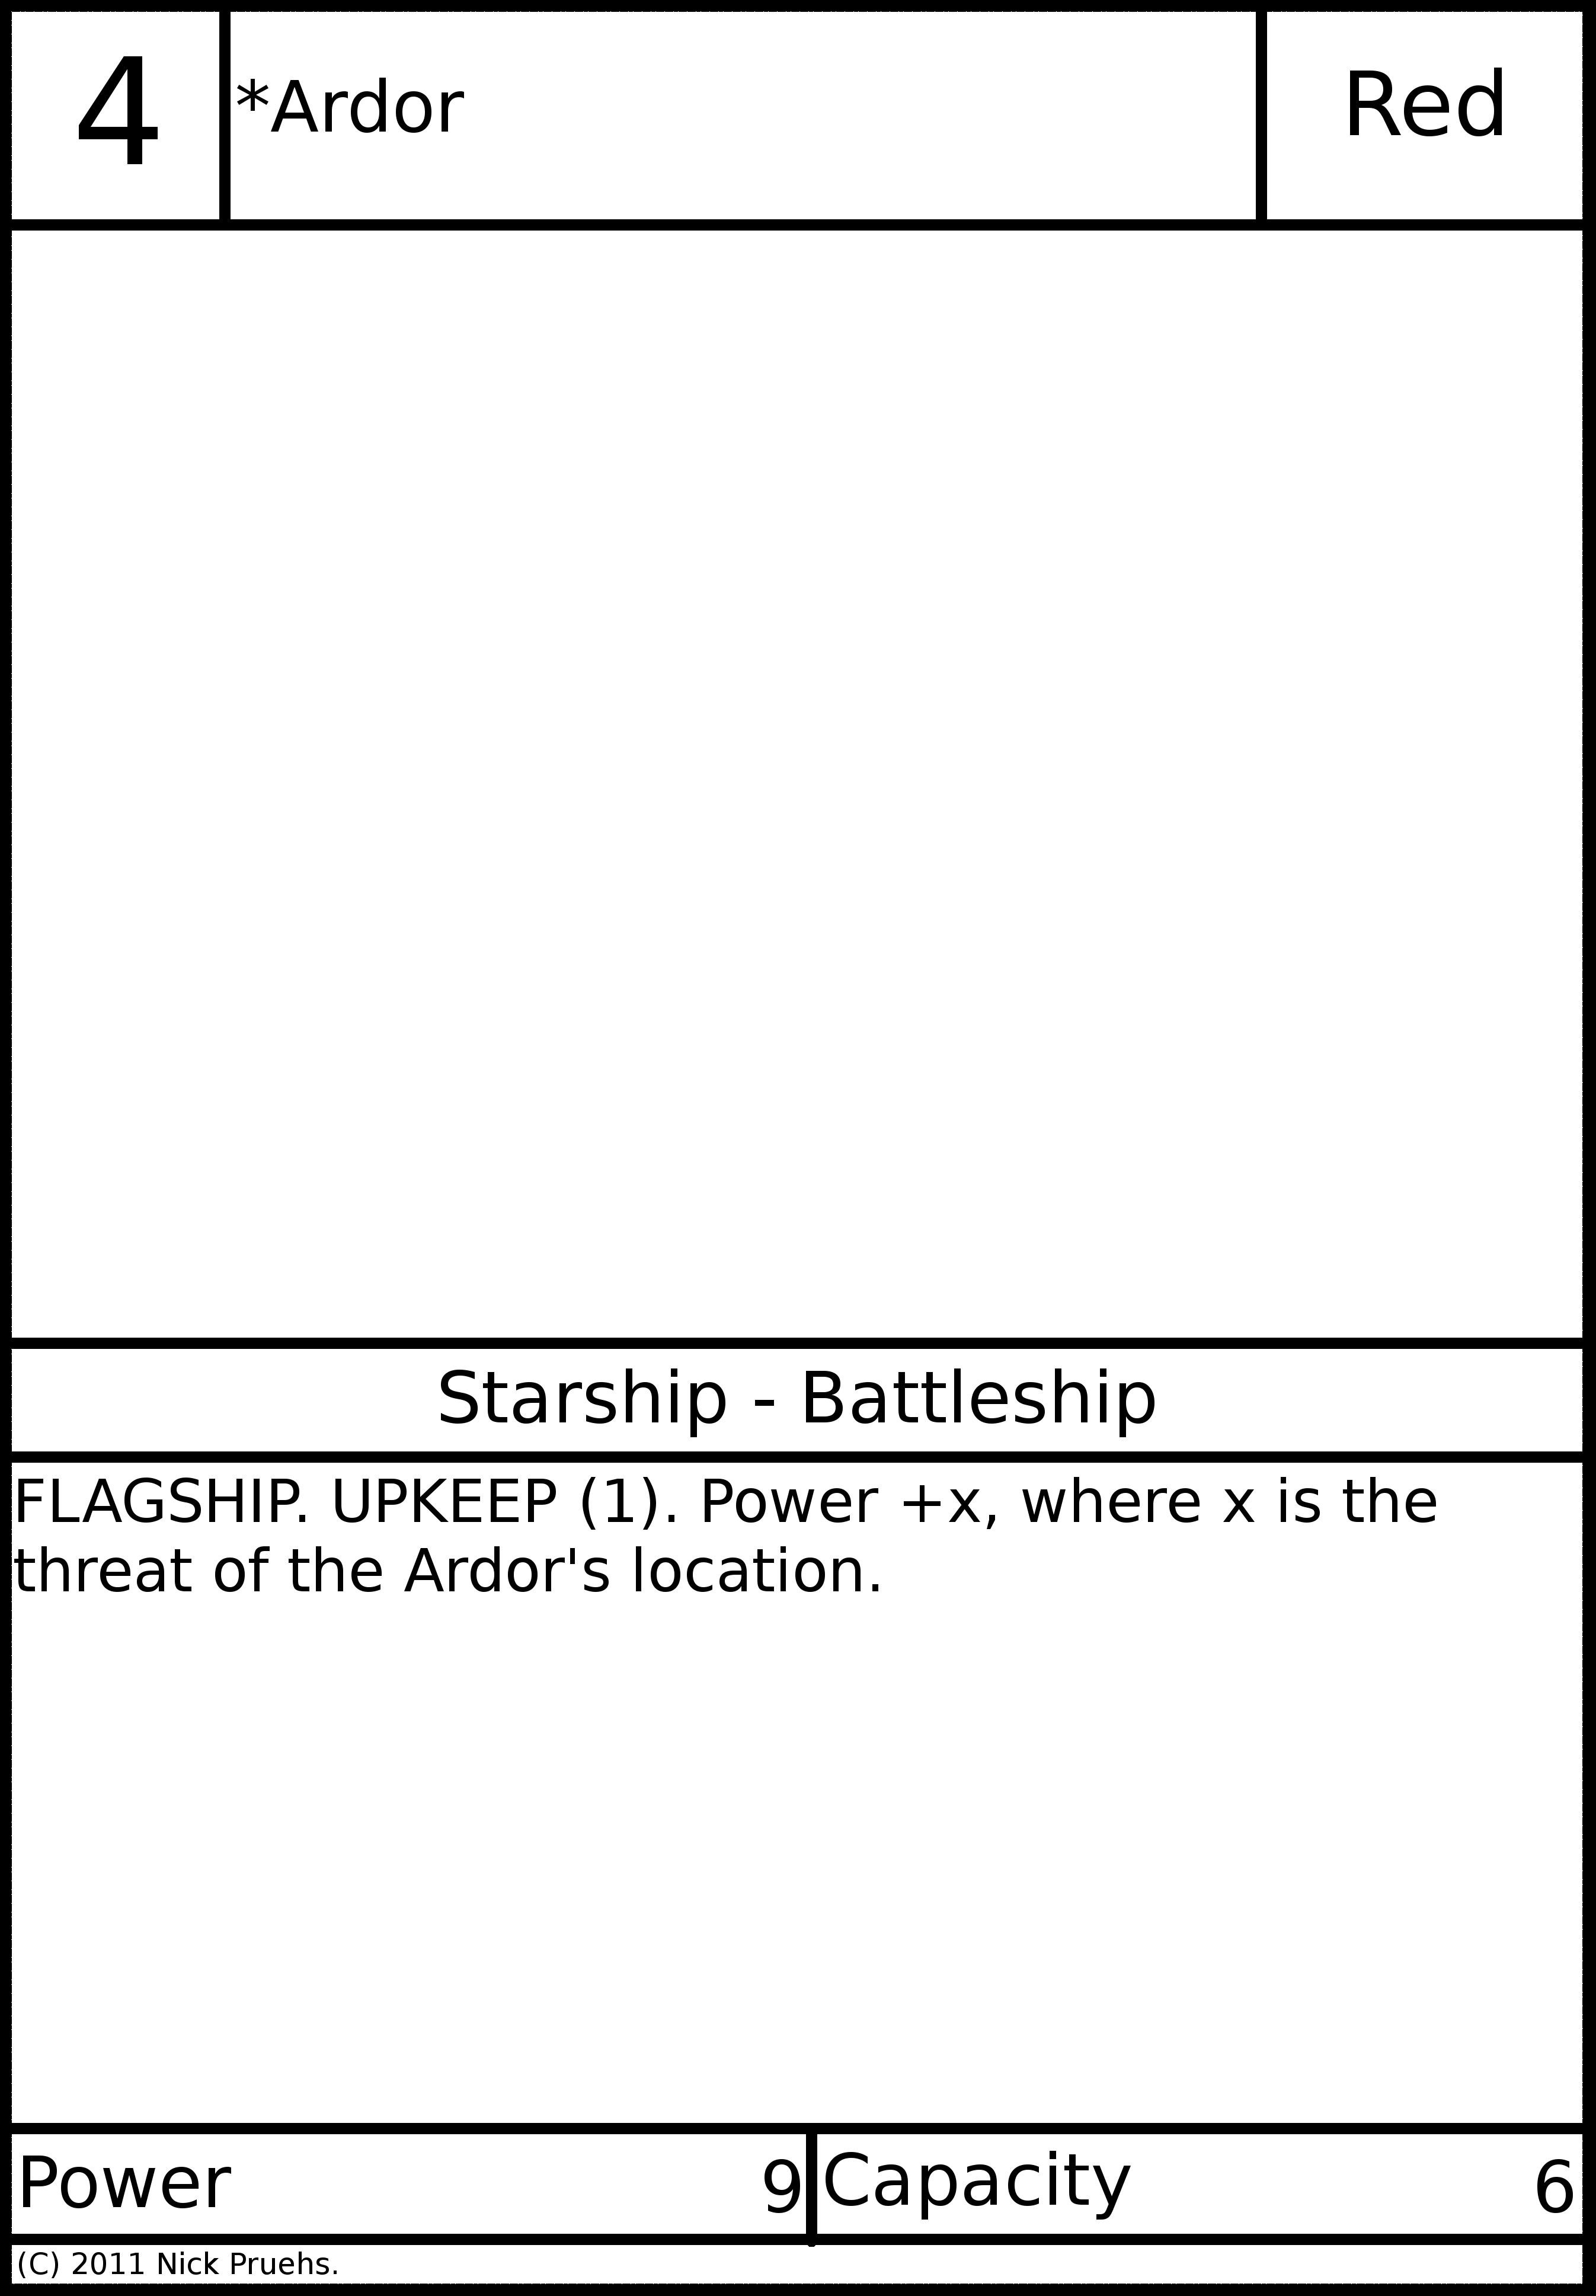
\includegraphics[width=0.5\textwidth]{examplestarship.png}
  \caption{A starship card.}
\end{figure}

No player may have more than three starships in play at any time (the limit for
Ac'arr players is six).

\subsection{Locations}

Location cards are used to illustrate the journey the player fleet makes. If
the players have covered a \emph{distance} of ten or more and survive the turn,
they win the game.

\begin{figure}
  \centering
  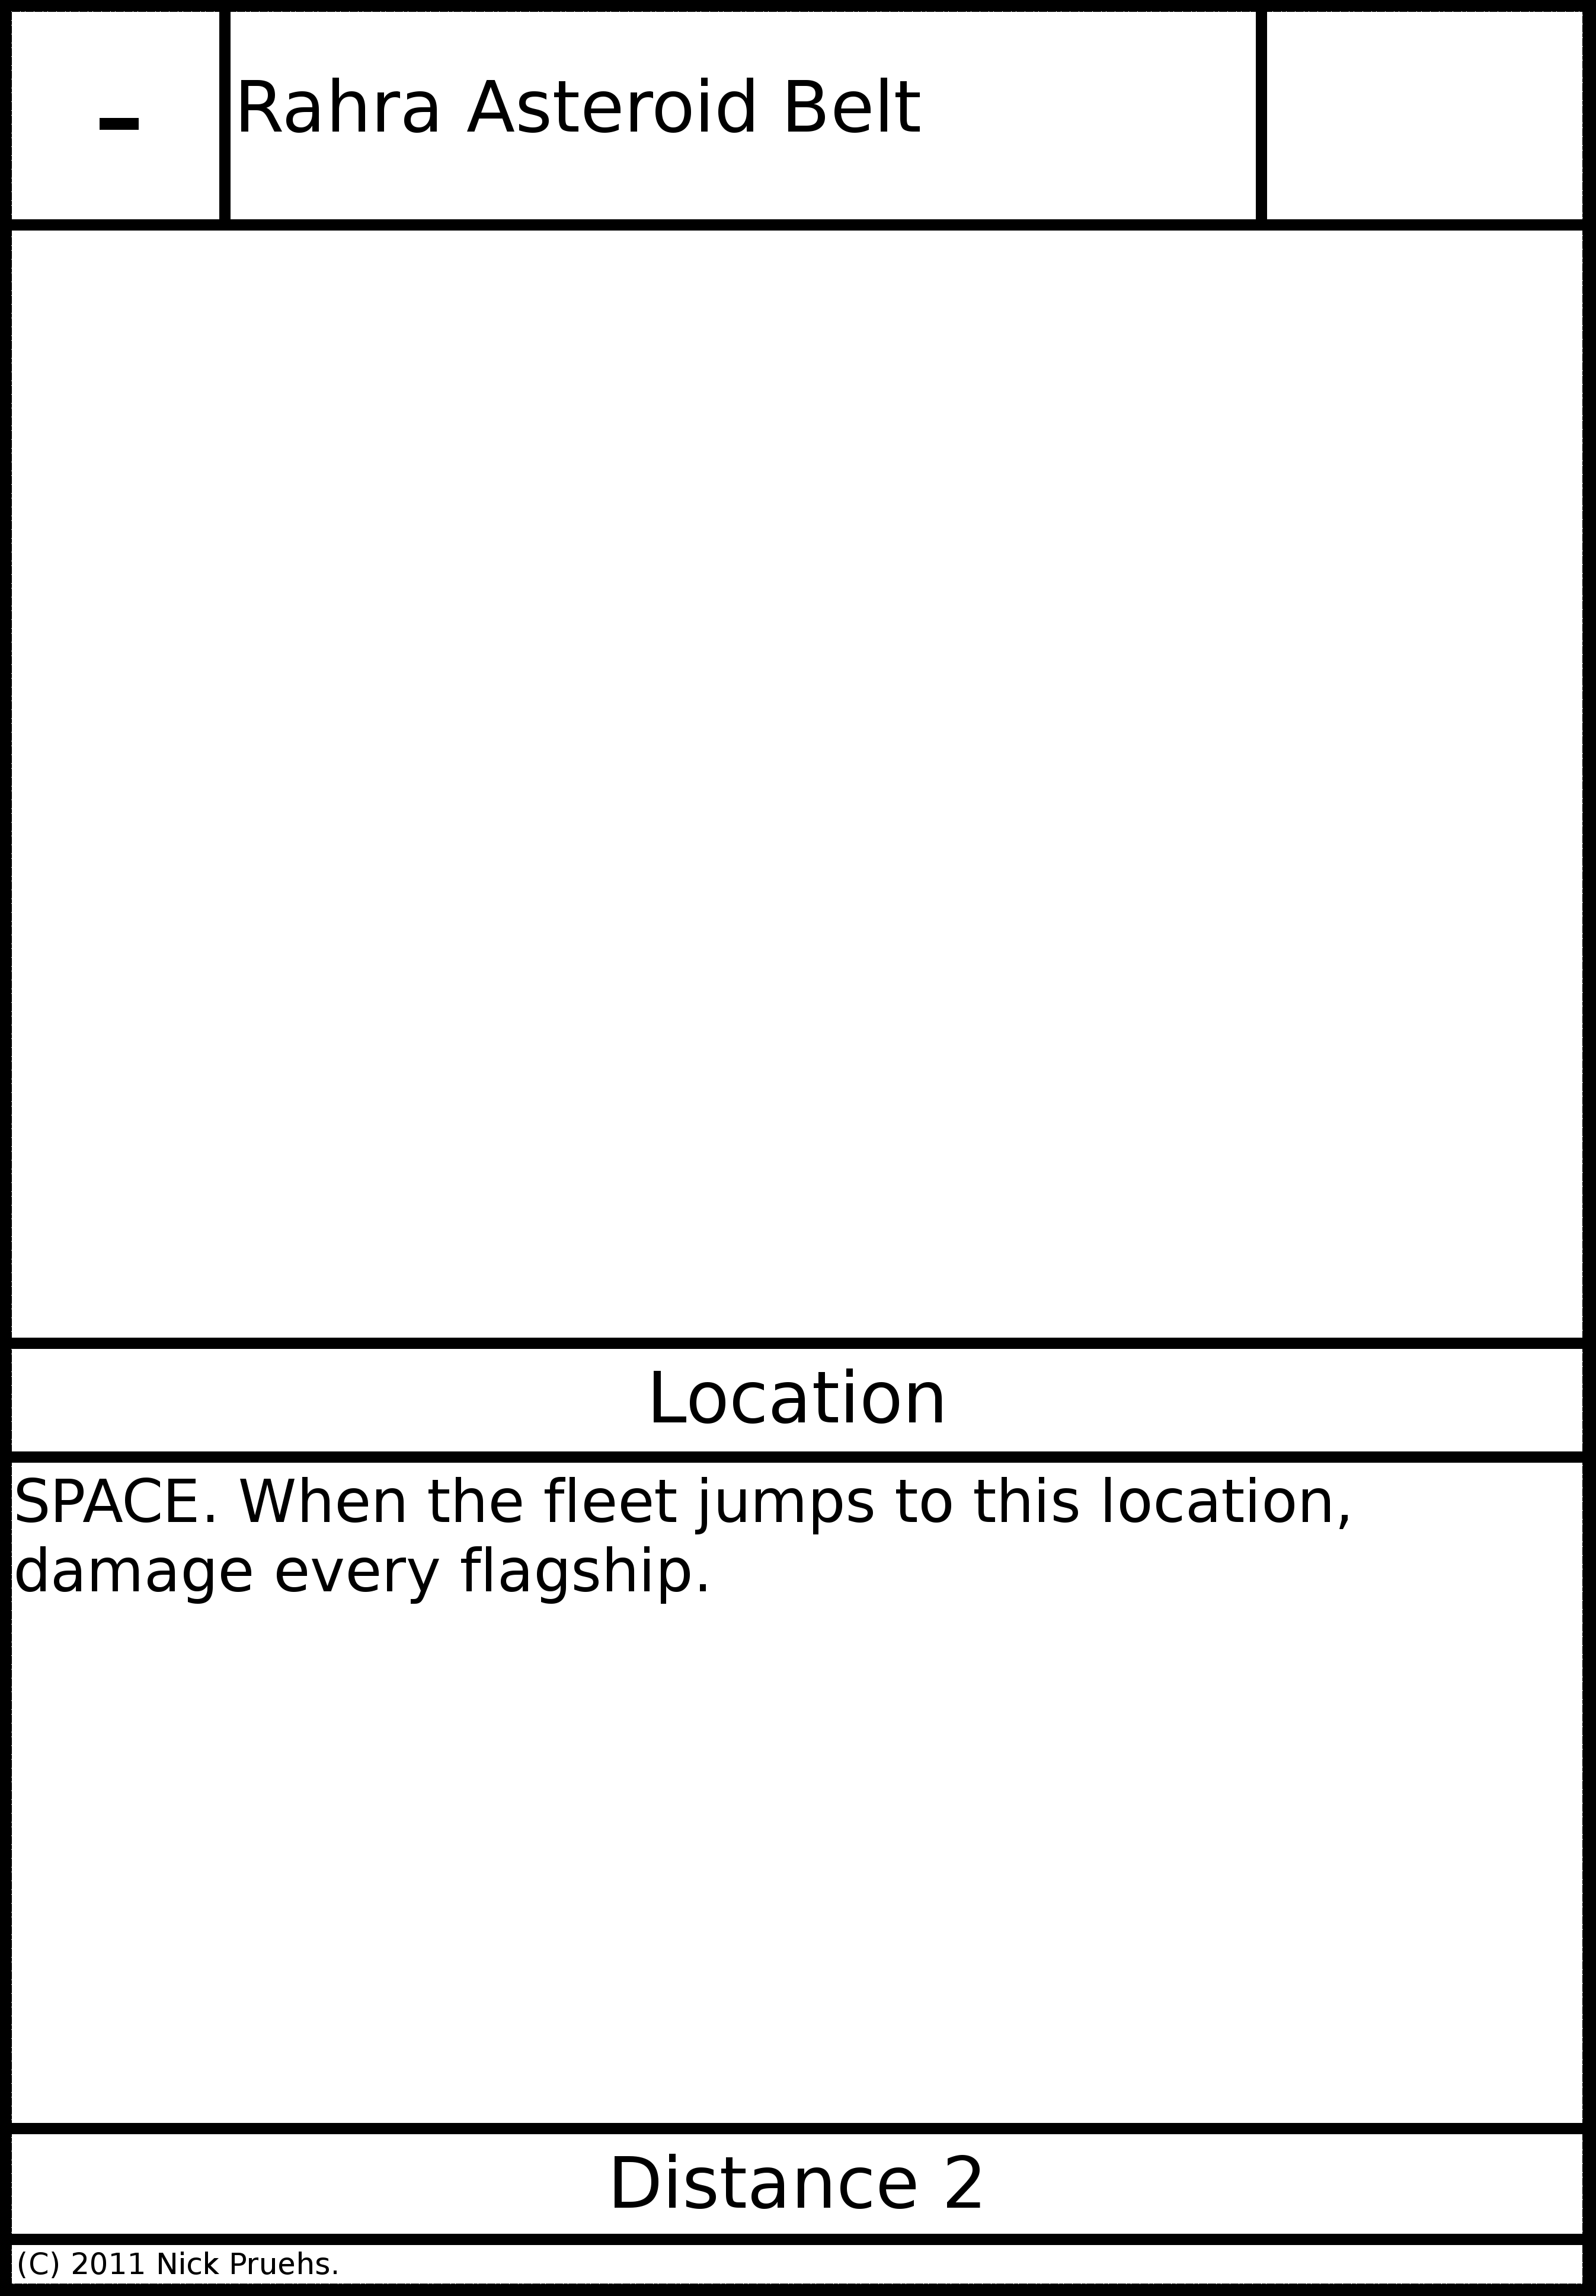
\includegraphics[width=0.5\textwidth]{examplelocation.png}
  \caption{A location card.}
\end{figure}

\subsection{Damage Cards}

Damage cards are put below damaged starships, reducing their power and capacity
values. Most damage cards have an additional effect, like preventing the ship
from overloading or from gaining any power bonuses.

\begin{figure}
  \centering
  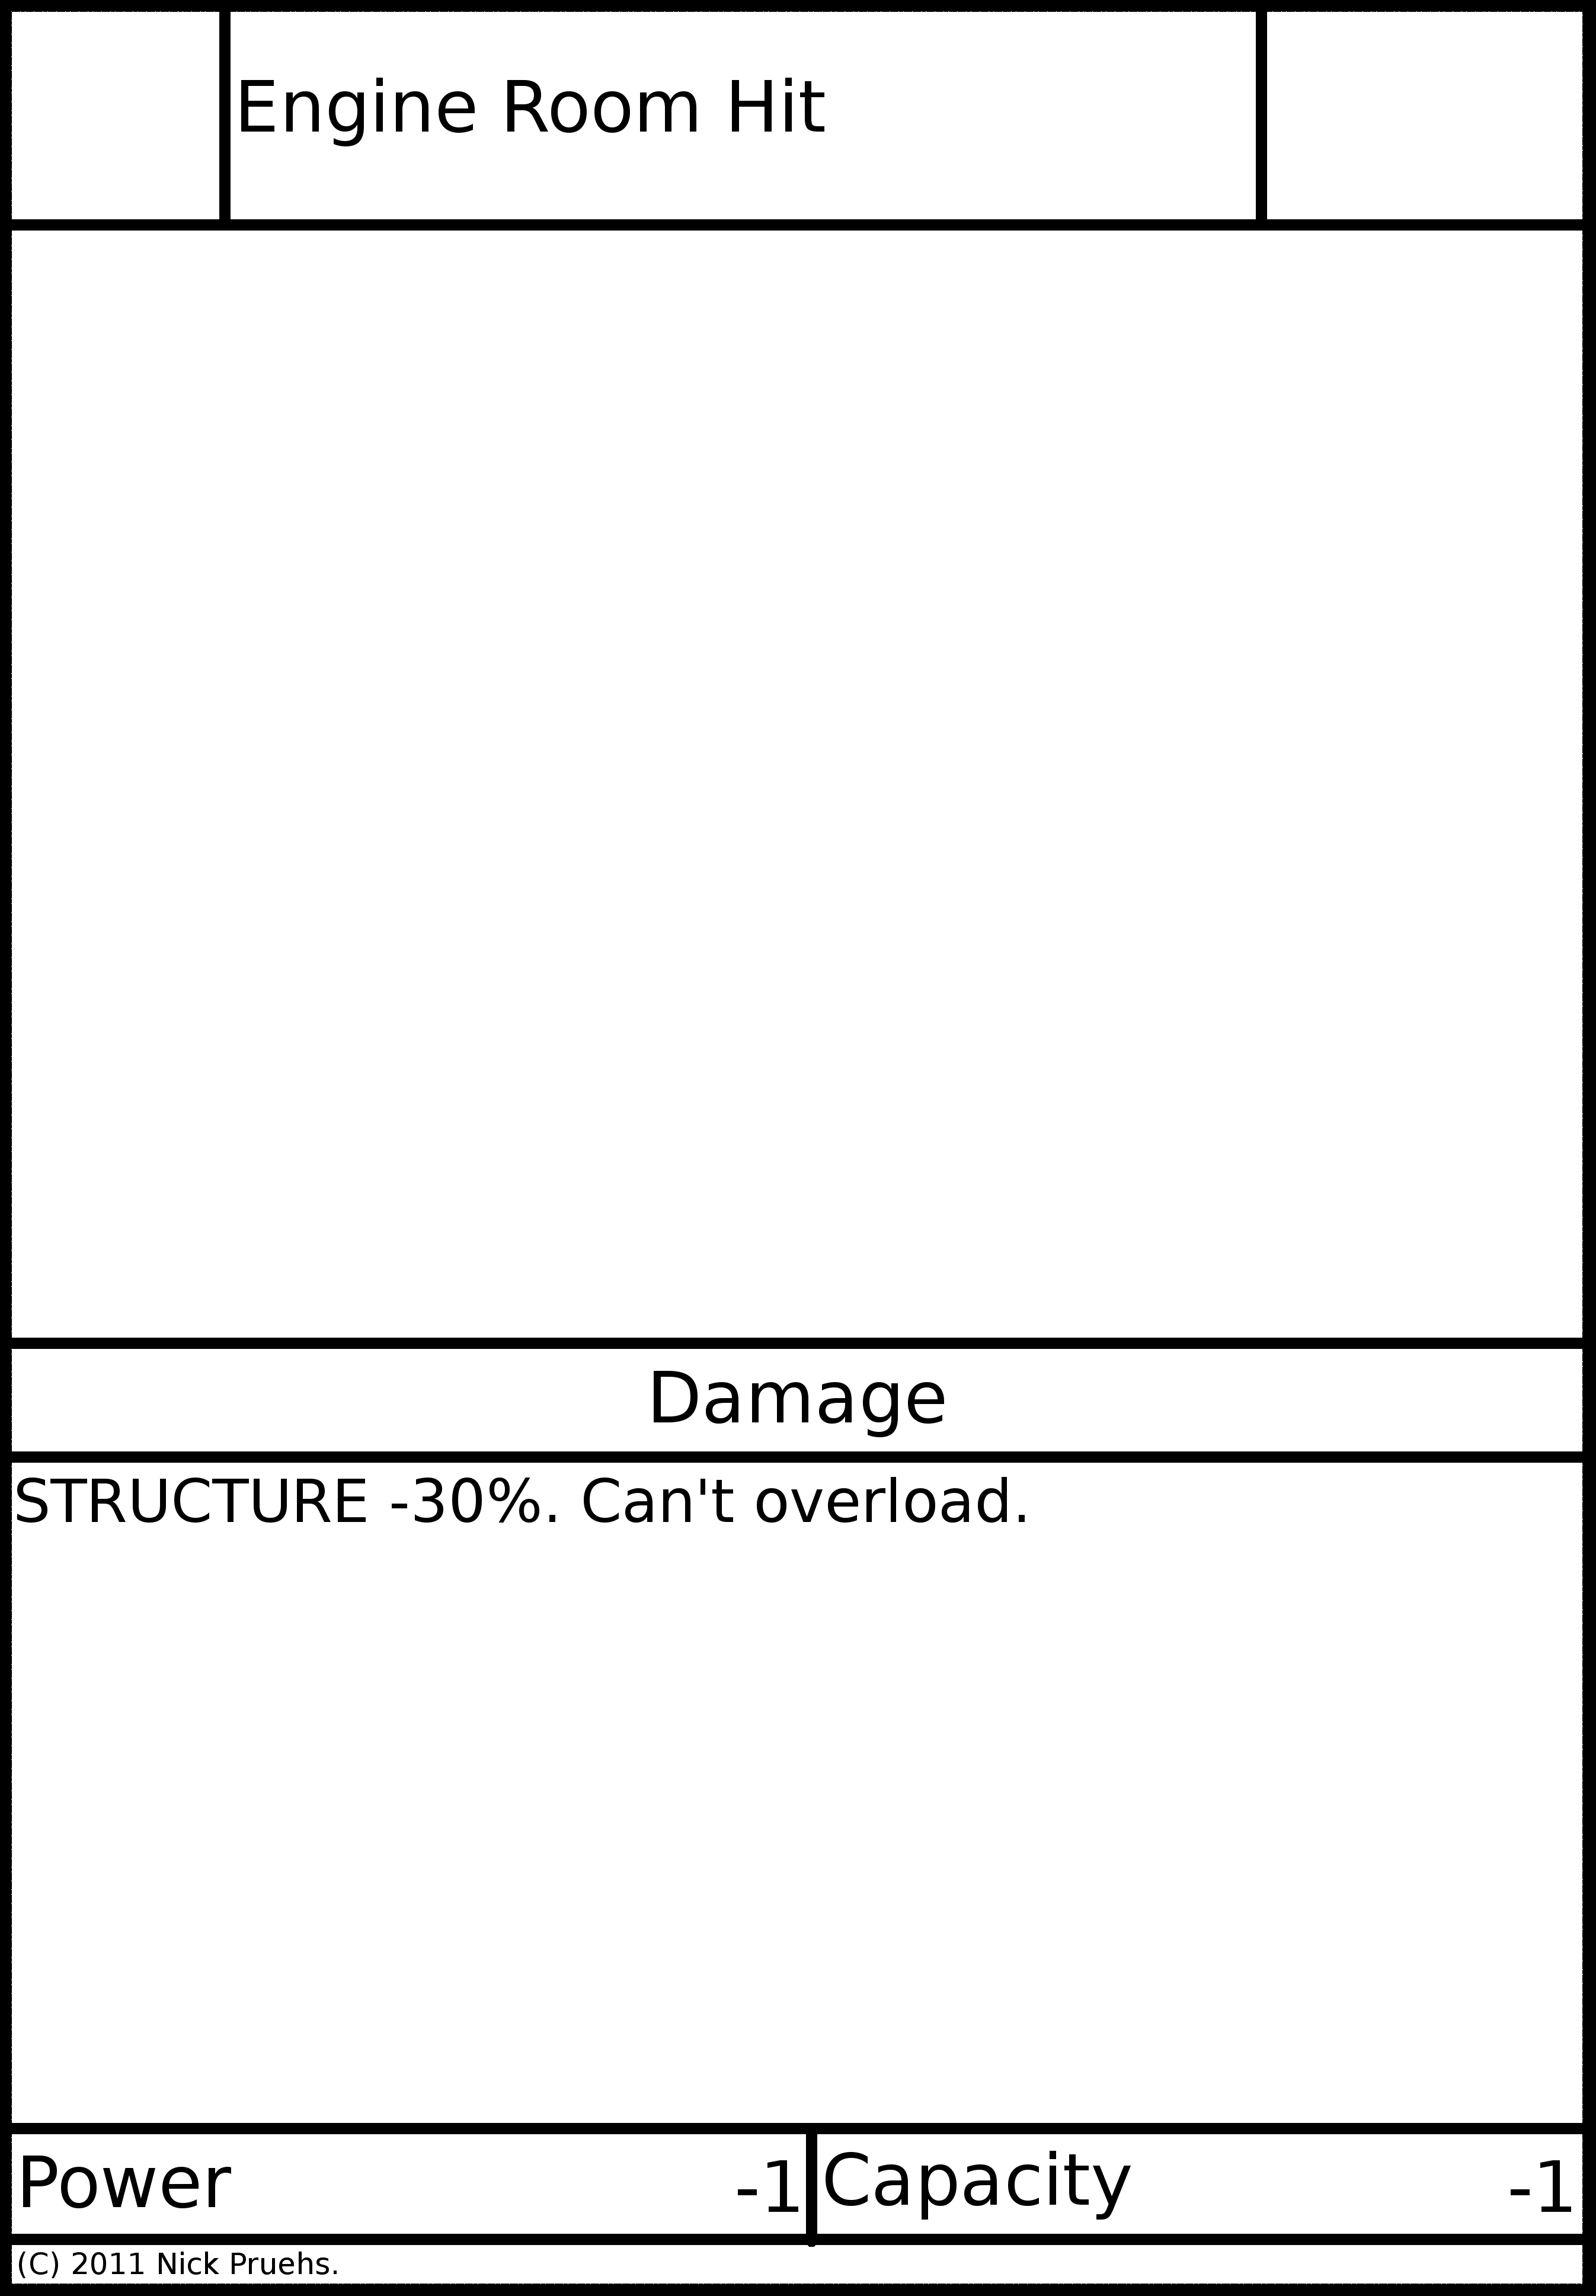
\includegraphics[width=0.5\textwidth]{exampledamage.png}
  \caption{A damage card.}
\end{figure}

\section{Turn Sequence}

All players play simultaneously.

\subsection{Main Phase}

Players may do each of the following things, in any order:

\begin{itemize}
 \item Deploy characters, starships and/or equipment, adding threat.
 \item Play effects and handle them, adding threat.
 \item Move characters and/or equipment between starships.
 \item Use special powers of any characters, starships and/or equipment cards.
\end{itemize}

\subsection{Jump Phase}

All players add threat equal to their starships' upkeep values (see subsection
\ref{upkeep}).

After that, the players reveal the top two cards of the location deck and pick
one location to jump to. The picked location is referred to as the
\emph{current location} of the player fleet, and its game text takes effect
immediately, replacing the game text of the previous location.

\subsection{Attack Phase}

At the beginning of the attack phase, add two threat for each location and one
threat for each player starship on the table.

Then, the players reveal cards from the top of the attack deck, one at a time,
removing their cost from the threat pool. If a card is revealed the cost of
which exceeds the number of tokens in the threat pool, the card is ignored and
discarded, and the players stop revealing cards.

\subsection{Assignment Phase}

Players assign their starships to the attackers according to the following
rules:

\begin{itemize}
 \item Every player starship must be assigned to defend against an attacker.
 \item If the number of player starships exceeds the number of attackers, the
remaining player ships may be assigned to join any fight, summing up their
power.
 \item If the number of attackers exceeds the number of player starships, the
remaining enemy ships are assigned one by one to the fights the enemies have
the lowest power in, in order of their power (lowest power ships first).
\end{itemize}

\subsection{Fight Phase}

The players resolve all fights, one at a time, in an order decided by them.
Each fight is resolved in a dedicated fight phase.

\begin{itemize}
 \item If the total power of all player ships is greater than the total power of
the enemy ships, the players win and the enemy ships are discarded.
 \item If the total power of the player ships is less than or equal to the total
power of the enemy ones, all player ships in that fight are \emph{damaged}: For
each ship damaged this way, the players draw a cards from the damage deck.
These cards take effect immediately. If the total number of characters and/or
equipment cards exceeds a damaged ship's capacity, they have to be discarded at
random until the capacity restrictions are met again. Damage cards remain until
the ship is repaired. As soon as the structure of a ship is reduced to 0, it is
destroyed.
 \item If the total power of the enemy ships in a fight is at least double the
total power of the player ones, the players are \emph{overpowered} and all of
their ships participating in that fight are destroyed immediately.
\end{itemize}

\subsection{Wrap-Up Phase}

Each player may discard any card and then draws cards until he or she has at
least four cards in the hand.

After that, all enemy ships are discarded. All tokens in the threat pool remain.

If the total distance covered by the players is ten or higher, the players win
the game.

\section{Keywords}
\subsection{Add or Remove (x)}
Every time a card tells a player to \emph{add (x)} or \emph{remove (x)}, he or
she adds or removes x tokens to or from the threat pool.

\subsection{Playing From The Draw Deck}
If a player is allowed to \emph{play a card from the draw deck}, he or she looks
through their deck for a copy of that card, puts that card into play adding its
cost to the threat pool, and shuffles his or her deck afterwards.

\subsection{Overload}

Some game texts may require the players to \emph{overload} a ship. This is done
by attaching the top card of the damage deck to that ship. Ships can be
destroyed by overloading them. Damage taken from overloading cannot be
prevented.

\subsection{Repair}

If a starship is \emph{repaired}, the players choose any attached damage
card to be discarded.

\subsection{Destiny}

If a ship is allowed to draw \emph{battle destiny}, the players reveal the top
card of the attack deck, add its threat to the ship's power and discard that
card.

\subsection{Upkeep}
\label{upkeep}

The \emph{upkeep} value of each player ship is added to the threat pool at the
beginning of each jump phase.

\subsection{Cloaking}

At the beginning of the attack phase, any number of ships with \emph{cloaking}
may choose not to participate in any fights.


\section{Other Important Rules}
\subsection{Uniqueness}

A small dot next to a card's name indicates that card is \emph{unique}: Unique
cards may not be deployed as long as any other copy of that card is in play or
in any destroyed pile.

\subsection{Spare Parts}

During the main phase, any player may discard a starship from hand to repair
a ship of the same type.

\section{Deck Construction Rules}

The minimum draw deck size is 30 cards. A deck must not contain any card more
than four times.

\section{Inspirations}

Fans will note that Pinned Down is clearly inspired by the Lord of the Rings
Trading Card Game by Decipher Inc., definitely the greatest trading card game
I've ever played. Credit must be paid.

The player fleets are led by a flagship of their choice and pass different
locations on their journey. Their ships are enhanced by equipment and effects,
and every time the players lose a fight, their ships get damaged and have to be
repaired. They can overload their ships to gain special benefits, and there's no
way of recovering destroyed ships at all. The stronger the players get, the
greater is the opposition they have to face as they advance.

The main difference between the two games is that Pinned Down is cooperative,
whereas Lord of the Rings obviously is not. Furthermore, there is no One Ring
in Pinned Down of course, and no similar mechanic to protect (or corrupt) the
flagship. Finally, there's no archery phase in Pinned Down, as all ships use
long-range weapons, and there are no ally cards - the players support each
other instead.

Other mechanics like cloaking ships, having them enhanced by their matching
commander or reducing their attributes by damage cards are derived from similar
mechanics in the Star Trek Customizable Card Game, another great trading card
game by Decipher. The initial version of Pinned Down contained some kind of
location spaceline and additional challenges to be solved using the teamwork
values of characters, too, but these mechanics have been removed because they
didn't really seem to add fun to the game. The focus of Pinned Down clearly is
on collaborating, on discussing decisions and planning the use of limited
resources, as well as finding clever ship fight assignments.

The terms battle destiny and upkeep are borrowed from the Star Wars Customizable
Card Game and Magic: The Gathering, respectively. Giving the players the chance
to choose the location to jump to pretty much works like in Battlestar
Galactica: The Board Game, and the idea of assigning different roles to the
players has been taken from Pandemic. Both are amazing (semi-)cooperative games
that led to the idea of creating this game.

\section{Design History}
\subsection{June 5, 2011}

\begin{itemize}
 \item No need for interrupts, as all players play simultaneously.
 \item Location affiliations are now part of the game text
(``A1 cards may be deployed here.'') Less icons required.
\end{itemize}

\subsection{June 6, 2011}

\begin{itemize}
 \item Attack location must be determined first in order to allow locations to
modify the attacker's threat costs.
\end{itemize}

\subsection{June 12, 2011}

\begin{itemize}
 \item Players may now redraw their initial hand if they have no starships at
all, reducing the difficulty at the beginning.
 \item Introduced Puppy Protection, reducing the difficulty at the beginning.
 \item Support firepower has been reduced to the total number of attacking ships
not assigned to a fight, reducing difficulty.
 \item Every ship now participates in only one fight per turn, reducing the
length of each turn. Bombardment happens if and only if there are no uncloaked
player ships left at the end of the attack phase.
 \item Bombardment damage has been reduced to the total number of bombarding
ships.
 \item Introduced fleets for easier handling of big numbers of ships and for
easier description of synergies.
 \item All fights are now 1v1, thus players can have support firepower, too,
simplifying assigning ships and resolving fights.
\end{itemize}

\subsection{June 13, 2011}

\begin{itemize}
 \item No longer adds location threat to the pool at the beginning of the attack
phase, simplifying the attack phase and reducing difficulty.
\end{itemize}

\subsection{June 26, 2011}

\begin{itemize}
 \item Locations turned out to be completely superfluous. A new location system
has been introduced: The players now reveal the top two cards of the location
deck after each main phase, and pick a location to jump to. The players win
if they cover a distance of ten or more. There's only one location deck in
total now. Characters, equipment and starships may deploy anywhere now. The
hyperspeed value of starships has been replaced by a capacity value that
restricts the total number of characters and/or equipment aboard. A location's
threat value is now added to the pool at the beginning of the attack phase
once again.
 \item Every player now starts with a flagship, and players may no longer
re-draw their initial hand. If all player flagships are destroyed, they lose
the game.
 \item Any time a player starship is damaged, two damage cards are drawn from
a new damage deck now, reducing the values of the damaged ship. Damage cards
can be removed by repairing a ship only, and if a ship is affected by too many
damage cards, it is destroyed.
 \item Challenges have been removed from the game. Similar cards are designed
using effect cards.
 \item Effects with cost greater than zero have to be played during the main
phase now, as players would avoid adding threat else.
 \item Fights are not 1v1 anymore again, as the impact of the support firepower
system on all other fights was far too strong. If the number of attacking
ships exceeds the number of defenders now, they're randomly assigned to
non-cloaked player ships.
\end{itemize}

\subsection{June 29, 2011}

\begin{itemize}
 \item Introduced destroyed piles for distinguishing discarded ship
cards from destroyed ships.
 \item Removed Puppy Protection as its effect is now granted by one of the
player flagships.
 \item Split the attack phase into three phases for easier reference by effect
timings.
 \item Added the spare parts rule that allows easier deck building.
 \item Removed teamwork from the game, as the game's focus is clearly on
fighting enemy ships and using effects and special powers to survive.
\end{itemize}

\subsection{July 1, 2011}

\begin{itemize}
 \item Players may not have more than five ships in their fleet, in order to
recude the length of each turn and assure that the game's scaling isn't broken.
 \item Assigining remaining enemy ships is now deterministic. Players should be
able to plan their fights.
 \item Added drawing battle destiny and upkeep mechanics.
 \item Added references to all games that inspired Pinned Down.
\end{itemize}

\subsection{July 13, 2011}

\begin{itemize}
 \item Tokens in the treat pool now remain at the end of the wrap-up phase in
order to increase difficulty.
 \item Further reduced the maximum number of ships per player fleet to reduce
the length of each turn. Reduced the maximum deck size accordingly.
\end{itemize}

\subsection{July 20, 2011}

\begin{itemize}
 \item Adds two threat per location on the table instead of the location threat
in order to increase opposition from turn to turn now. Location threat has
become superfluous.
\end{itemize}

\newpage

\appendix

\section{Turn Sequence}

\begin{enumerate}
 \item Main Phase

 \begin{itemize}
  \item Deploy characters, starships and/or equipment.
  \item Play effects.
  \item Move characters and/or equipment between starships.
  \item Use special powers.
 \end{itemize}

 \item Jump Phase

 \begin{enumerate}
  \item Add upkeep threat.
  \item Pick destination location.
 \end{enumerate}

 \item Attack Phase

 \begin{enumerate}
  \item Add (2) for each location and (1) for each starship on the table.
  \item Play attack ships and events.
 \end{enumerate}

 \item Assignment Phase
 \item Fight Phase
 \item Wrap-Up Phase

 \begin{enumerate}
  \item Each player may discard a card.
  \item Each player draws cards until he or she has at least four cards in his
or her hand.
  \item Discard all enemy ships.
  \item If the total distance covered is ten or higher, the players win.
 \end{enumerate}

\end{enumerate}


\end{document}
